% !TEX encoding = UTF-8
% !TEX TS-program = pdflatex
% !TEX root = ../tesi.tex

%**************************************************************
\chapter{L'azienda}
\label{cap:azienda}

\section{Descrizione}

WorkWave, una divisione di IFS, è una società americana fondata nel 1984 che fornisce soluzioni di Field Service Management e che connette ogni aspetto del business attraverso le sue piattaforme unificate e di facile uso. L'insieme delle soluzioni della compagnia permettono facilmente ai professionisti del settore di assegnare ed automatizzare attività di vendita e marketing, migliorando l'efficienza ed incrementando il monitoraggio sulle operazioni sul campo attraverso soluzioni mobile. \\

Le piattaforme di WorkWave forniscono ad oltre 8 mila clienti un livello senza precedenti di analisi del business, permettendolo loro di aumentare l'efficienza, il guadagno e garantendo un'eccezionale customer experience.

\begin{figure}[H] 
  \centering 
  
\includegraphics[]{workwave-logo} 
  \caption{Logo dell'azienda WorkWave}
\end{figure}

\section{Servizi offerti}

WorkWave aiuta aziende nel campo Field Service Management, oltre che industrie di trasporti e logistica, a mitigare gli aspetti dolorosi che incontrano ogni giorno. Consente loro infatti di salvare tempo, spese e migliorando il servizio agli utenti. \\

Per Field Service Management si intendono risorse impiegate per instradare verso i domicili dei clienti, quali localizzazione dei veicoli, gestione delle attività degli operatori, pianificazione ed impiego delle attività, garanzia della sicurezza dei conducenti ed integrazione di tali funzionalità con depositi, fatturazione ed altri servizi back-office. \\

WorkWave fornisce a tale scopo sia soluzioni per l'installazione e manutenzione hardware che servizi software per l'aiuto della gestione di tali attività. \\

La suite dei servizi software cloud, mobile e marketing permette a compagnie di ogni dimensione di facilmente stimare attività, pianificare ed dirigere operatori mobili con facilità. Di seguito si elencano i principali prodotti correlati all'attività di stage:

\begin{itemize}
  \item \textit{WorkWave Service}: è un servizio software che consente di velocemente schedulare rotte efficienti, visionare la produttività in tempo reale degli operatori, visualizzare stime e gestire pagamenti;
  \item \textbf{WorkWave Route Manager}: è un set di servizi per la gestione dei veicoli al fine di migliorare l'efficienza e la scalabilità attraverso pianificazione dinamica e miglioramenti intelligenti delle rotte. L'algoritmo proprietario del Route Manager garantisce che le migliori rotte per gli operatori siano usate per salvare tempo, costi e migliorare la soddisfazione dei clienti;
  \item \textit{WorkWave GPS}: fornisce un'intuitiva panoramica dei propri veicoli e delle propie risorse con un potente servizio GPS che cattura le azioni dell'operatore e le posizioni in tempo reale dei veicoli. Permette inoltre di migliorare la sicurezza dei guidatori, segnalare comportamenti errati e riportare incidenti.
\end{itemize}

\section{Route Manager}

\begin{figure}[h] 
  \centering 
  
\includegraphics[width=0.5\columnwidth]{workwave-route-manager-logo} 
  \caption{Logo WorkWave Route Manager}
\end{figure}

\textit{WorkWave Italy} è la sede centrale europea di WorkWave, dove sono concentrati gli sviluppi dell'algoritmo di routing e del prodotto Route Manager, contesto di sviluppo delle attività descritte in questo documento. \\

\textbf{WorkWave Route Manager} invece automatizza la pianificazione delle rotte per migliorare l'efficienza e la comunicazione tra l'amministrazione ed i guidatori dei veicoli, in maniera completamente customizzabile tramite le sue API. \\

\begin{figure}[H] 
  \centering 
  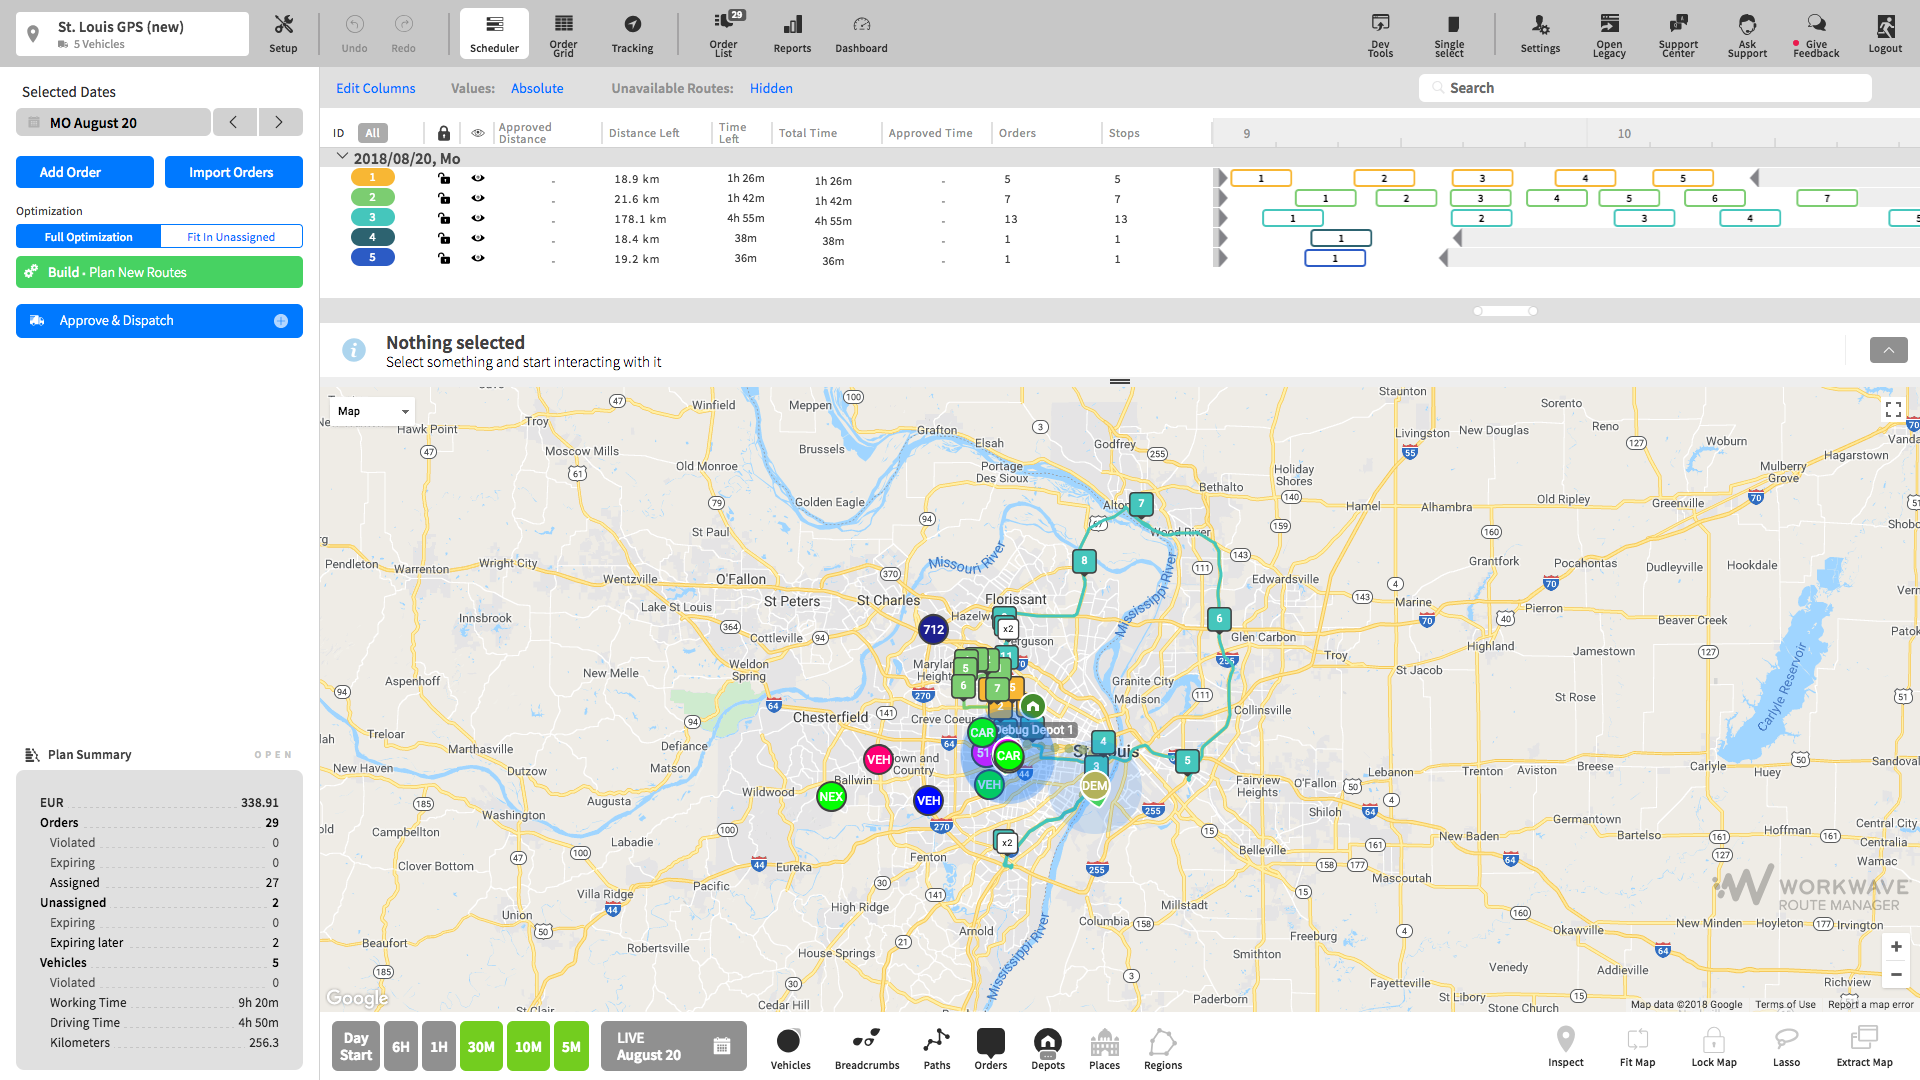
\includegraphics[width=1\columnwidth]{route-manager} 
  \caption{WorkWave Route Manager}
\end{figure}

In particolare, per quanto riguarda routing \& scheduling, rende possibile navigare attraverso gli orari di ricezione, schedulare le attività dei guidatori giornalmente ed eseguire report sulle performance. Attraverso le impostazioni, il software fornisce rotte ottimali in base ai propri vincoli stradali. \\

È inoltre possibile fare aggiustamenti manuali alle rotte via drag\&drop, approvare i piani e mandarli in esecuzione agli operatori sui veicoli. Oltre a ciò consente di visualizzare istantaneamente gli effetti delle modifiche sul numero di ordini possibili per i veicoli disponibili, il tempo stimato di completamento delle attività e comparare il costo per miglio.

\begin{figure}[H] 
  \centering 
  
\includegraphics[width=1\columnwidth]{rm-scheduler} 
  \caption{WorkWave Route Manager - Scheduler degli ordini}
\end{figure}
